\documentclass[a4paper,10pt]{article}
\usepackage[latin1]{inputenc}
%\usepackage{color}
%\usepackage{colortbl}
%\usepackage{amstext}
\usepackage{amsmath}
%\usepackage{graphicx}
\usepackage{pgfplotstable}

\makeatletter
\makeatother

\begin{document}

\title{Tragfl�chenmodell im Windkanal}
\author{Andreas Zuber, Florian Schnider}

\maketitle

\section{Einleitung}
Anhand eines Tragfl�chenmodells sollen die Grundlagen der Fluiddynamik untersucht werden.

\subsection{Versuchsaufbau}\label{sec:versuchsaufbau}
% - Skizze
% - Ger�tenummern
% ...
\begin{center}
 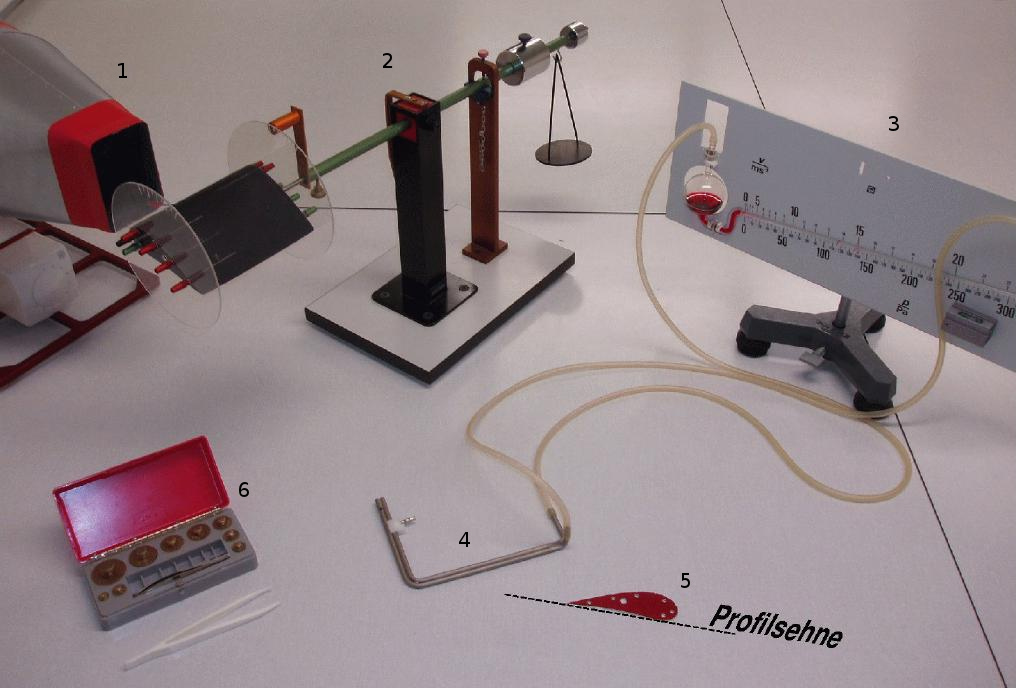
\includegraphics[scale=0.4]{./versuch_07_windkanal_aufbau.jpeg}
 % versuch_07_windkanal_aufbau.jpeg: 1016x688 pixel, 84dpi, 30.72x20.80 cm, bb=0 0 871 590
\end{center}

\subsection{Material}
\begin{enumerate}
\item Windmaschine/Turbine (EP A 05-1739)
\item Tragfl�chenmodell
\item Manometer (EP A 05 1076)
\item Drucksonde
\item Fl�gelprofilsehne
\item Set mit Gewichten 
\end{enumerate}

\section{Theorie}\label{theorie}
% - Zusammenfassung und Zusammenstellung der f�r die Auswertungben�tigten Formeln
Gewicht- und Antriebskraft Berechnung f�r Aufgabe 1:
\[F_a=\Delta m_1 g\]
\[F_\omega=\Delta m_2 g\]

\section{Praktische Aufgaben}
% - Alle Messwerte in �bersichtlichen Tabellen mit Mittelwerten und Fehlerangaben
\subsection{Aufgabe 1}
Die erste Aufgabe war f�r eine bestimmte Str�mungsgeschwindwigkeit ein Polardiagramm
der Kr�fte zu erstellen. Dazu waren zwei Messungen notwendig.

Zuerst mussten wir die Gewichtskraft des Tragfl�chenmodells aufheben. Auf der Seite mit
der Schale f�r die Gewichte befindet sich ein zus�tzliches verstellbares Gewicht welches wir
so einstellen mussten das wir zus�tzliche Gewichte aus dem Geichtsset auf die Schale legen konnten.
Dies erm�glicht es w�rend der Messung Gewichte zu entfernen und aus der Differenz die Auftriebskraft
abzulesen.

\begin{itemize}
 \item Str�mungseinstellung an Turbine: 9
 \item Gewichte in Schale in balance: 80g
\end{itemize}

Das Tragfl�chenmodell ist so ausgelegt das mit den Gewichten direkt die Kraft auf die
Tragfl�che gemessen werden kann. Die Kr�fte an der Tragfl�che erzeugen ein Drehmoment welches wir
mit den Gewichten kompensieren.

F�r die Anstellwinkel $\phi$ haben wir 0\textdegree in der Ausgangslage. Negative Winkel sind Drehungen im
Uhrzeigersinn, positive im Gegenuhrzeigersinn.

Bei der Messung von $F_a$ wird die Auftriebskraft der Tragfl�che gemessen. Dazu wird die Tragfl�che
horizontal angeblasen.

\begin{center}
\begin{tabular}{|c|c|c|c|}
\hline
$\phi$ [\textdegree]& $m_2$ [kg]& $\Delta m_1$ [kg] & $\left| F_a\right|$ [N] \\
\hline
-20 &0.005 &-0.075 &0.736 \\
\hline
-15 &0.015 & -0.065 &0.638 \\
\hline
-10 &0.025 & -0.055 & 0.54\\
\hline
-5 & 0.04& -0.04 & 0.392\\
\hline
0 &0.05 & -0.03 &0.294 \\
\hline
5 & 0.061& -0.019 & 0.186\\
\hline
10 &0.07 & -0.01 & 0.098\\
\hline
15 &0.082 & 0.002 &0.02 \\
\hline
20 &0.094 & 0.014 & 0.137\\
\hline
\end{tabular}
\end{center}

F�r die Messung von $F_\omega$ mussten wir die Turbine auf den Boden stellen. Die
Tragfl�che wurde um 90\textdegree gedreht. So konnten wir direkt die Wiederstandskraft
auf die Tragfl�che messen.

\begin{center}
\begin{tabular}{|c|c|c|c|}
\hline
$\phi$ [\textdegree]& $m_2$ [kg]& $\Delta m_2$ [kg] & $\left| F_\omega\right|$ [N] \\
\hline
20&0.047&-0.033&0.32373 \\
\hline
15&0.053&-0.027&0.26487 \\
\hline
10&0.057&-0.023&0.22563 \\
\hline
5&0.056&-0.024&0.23544 \\
\hline
0&0.062&-0.018&0.17658 \\
\hline
-5&0.063&-0.017&0.16677 \\
\hline
-10&0.062&-0.018&0.17658 \\
\hline
-15&0.063&-0.017&0.16677 \\
\hline
-20&0.062&-0.018&0.17658 \\
\hline
\end{tabular}
\end{center}

Die so gemessenen Kr�fte haben wir in ein Diagramm eingezeichnet. Die Verbindungslinie ist
lediglich dazu da den Verlauf der Kurfe besser zu erkennen. F�r die Messung relevant sind
lediglich die Punkte.

\begin{center}
 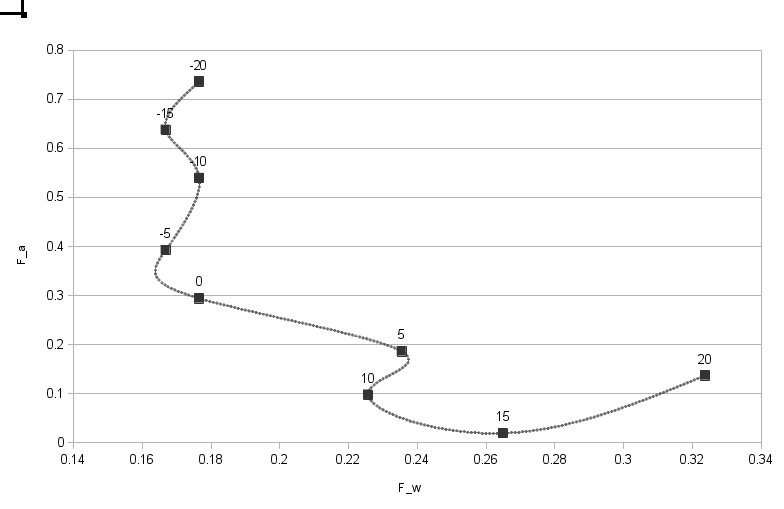
\includegraphics[scale=0.5]{./versuch_07_graph1.jpeg}
 % versuch_07_graph1.jpeg: 784x509 pixel, 84dpi, 23.71x15.39 cm, bb=0 0 672 436
\end{center}

\subsection{Aufgabe 2}

\subsubsection{Teilaufgabe 2a}
Bei dieser Teilaufgabe w�hlen wir direkt ein Resultat aus der ersten Ausgabe aus welches wir
weiter verwenden:

\[\phi=-15\textdegree \Longrightarrow F_a=0.638N\]

\subsubsection{Teilaufgabe 2b}
Bei dieser Aufgabe haben wir Die Druckverteilung um das Profil herum gemessen. Die Tragfl�che
war bei dieser Messung fix in der in Teilaufgabe 2a gew�hlten Position.



\section{Diskussion}
% - Kommentare
% - Vergleich der Messwerte mit Theorie und Literaturwerten
% - Hinweis auf m�glich Fehlerquellen (besonders systematische Fehler)
% - Schwierigkeiten bei der Messung
% ...


\begin{thebibliography}{99}

\bibitem{Script} Anleitung zum Physikpraktikum, Praktikumsskript FS 2012, P. Wurz

\end{thebibliography}

\end{document}